\documentclass[12pt]{article}

\usepackage{mathtools}

% \usepackage[margin=1in]{geometry}

\newcommand*{\eu}{e}
\newcommand*{\iu}{i}

\DeclarePairedDelimiter{\bra}{\langle}{\rvert}
\DeclarePairedDelimiter{\ket}{\lvert}{\rangle}
\DeclarePairedDelimiterX{\braket}[2]{\langle}{\rangle}
  {#1\,\delimsize\vert\,\mathopen{}#2}

\usepackage{biblatex}
\addbibresource{report.bib}

\usepackage[hidelinks]{hyperref}

\title{The Quantum Ising Chain as an Open Quantum System}
\author{David Basoco \and Jack Hetherington \and Davis Rash \and Tim Ross}
\date{December 6, 2023}

\begin{document}
  \maketitle


  \section{Introduction}

The transverse-field Ising model is a quantum mechanical model of a spin lattice, and can be simulated on a quantum computer. The Hamiltonian of the Ising Model is given by 
\begin{equation}
    \label{eq:hamiltonian}
    H = \sum_{i = 1}^{n} \sigma_{i}^{x} \sigma_{i + 1}^{x}
        + \sigma_{1}^{y} \sigma_{2}^{z} \dotsm \sigma_{n - 1}^{z} \sigma_{n}^{y}
        + \lambda \sum_{i = 1}^{n} \sigma_{i}^{z},
  \end{equation}
 The system being studied in this project is an Ising model structured in a loop with 8 sites.
 The magnetization of the full Ising model can be evolved over time, to analyze the effects of changes to parameters. Since no quantum system can be perfectly isolated from the environment, the system will be coupled to an environment at a single site. The system is represented in Fig.~\ref{fig:SystemDiagram}.
\begin{figure}[!htb]
    \centering
    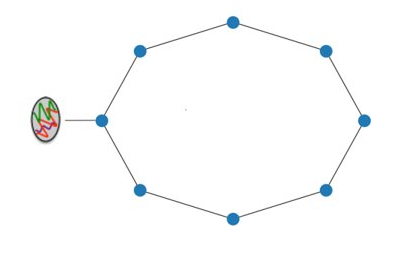
\includegraphics[width=\textwidth]{images/SystemDiagram.png}
    \caption{Representation of the system being studied.%
      \label{fig:SystemDiagram}}
  \end{figure}
Due to limitations of using the IBM quantum systems, and the large number of runs needed to get necessary data, the IBM QASM simulator was used for this project. 

  \subsection{Applications}

No quantum system is perfectly protected from the environment. Simulating the Ising model, with a known result, can provide information on what kinds of noise are present in an untested quantum computer. Each type of noise affects the Ising model, some examples include the amplitude damping channel causes a shift down in the total magnetization and the depolarizing channel causes the magnetization to decay over time. This will let us determine the exact type(s) of noise affecting the system.

  \section{Quantum Gate Operations}
 To solve the Ising model on a quantum computer, we need to diagonalize Eq.~\eqref{eq:hamiltonian}. We do this by applying a unitary disentangling operator \( U_{\textnormal{dis}} \) such that
  \begin{equation}
    \tilde{H}
      = U_{\textnormal{dis}}^{\dagger} H
        U_{\textnormal{dis}}^{\vphantom{\dagger}},
  \end{equation}
  where \( \tilde{H} \) is a noninteracting Hamiltonian. For the Ising model, the method to obtain the \( U_{\textnormal{dis}} \) is threefold.
  \begin{enumerate}
   \item We first need to map spins to fermionic modes with the Jordan--Wigner transform. If this step is required varies depending on the hardware involved, in our case it was not required.
   \item Then we need to get the fermions in moment space by applying the Quantum Fourier transform.
   \item Finally, we perform the Bogoliubov transform to decouple the modes in opposite momenta.
  \end{enumerate}
  This gives us the three-step recipe for our unitary disentangling operator, which is the same for all qubit counts.
  \begin{equation}
    U_{\textnormal{dis}}
      = U_{\textnormal{JW}} U_{\textnormal{FT}} U_{\textnormal{Bog}}.
  \end{equation}

  \subsection{Quantum Fast Fourier Transformation}

  \subsection{Bogoliubov Transformation}

  \section{Time Evolution}

  \section{Open Quantum Decoherence Channels}

  \subsection{Amplitude Damping Channel}

  \subsection{Depolarizing Channel}
The depolarization channel applied over time will move the system into an $\frac{I}{2}$ state. The rate of this decoherence is affected by a decay-rate parameter $\gamma$, which was kept constant at 0.5 for all runs. As shown by the following graph, the magnetization of the system decreases over time while coupled to the system. Since the depolarizing channel is only coupled at a single site, the decrease in energy applied to the single site must be propagating through the system and decreasing the magnetization of the whole system, but the affect of the transverse field prevents the system from going all the way into the $\frac{I}{2}$ state. The three values of $\lambda$ were graphed with the depolarizing channel, as shown in the figures. The effect of the depolarization channel is most noticeable with the higher value of $\lambda$, see Fig.~\ref{fig:DepolChannelLambda18},  but the decrease in magnetization can also be seen in the lower $\lambda$s in Fig.~\ref{fig:DepolChannelLambda05} and Fig.~\ref{fig:DepolChannelLambda09} .

\begin{figure}[!htb]
    \centering
    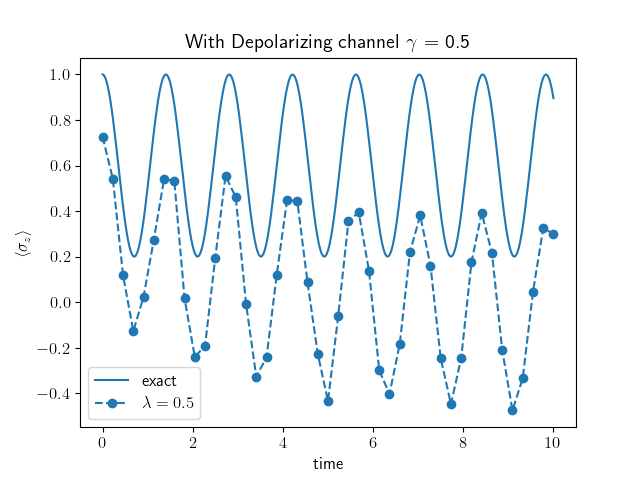
\includegraphics[width=\textwidth]{images/DepolChannelLambda05.png}
    \caption{Time evolution of the Ising model coupled to a depolarizing channel with $\lambda$ = 1.8%
      \label{fig:DepolChannelLambda05}}
  \end{figure}

\begin{figure}[!htb]
    \centering
    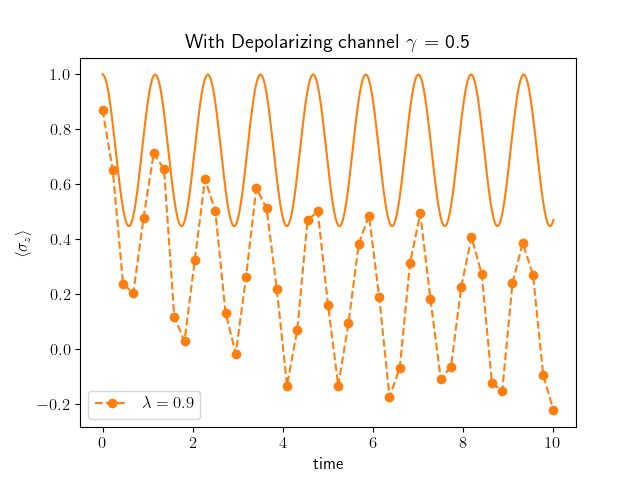
\includegraphics[width=\textwidth]{images/DepolChannelLambda09.png}
    \caption{Time evolution of the Ising model coupled to a depolarizing channel with $\lambda$ = 1.8%
      \label{fig:DepolChannelLambda09}}
  \end{figure}

\begin{figure}[!htb]
    \centering
    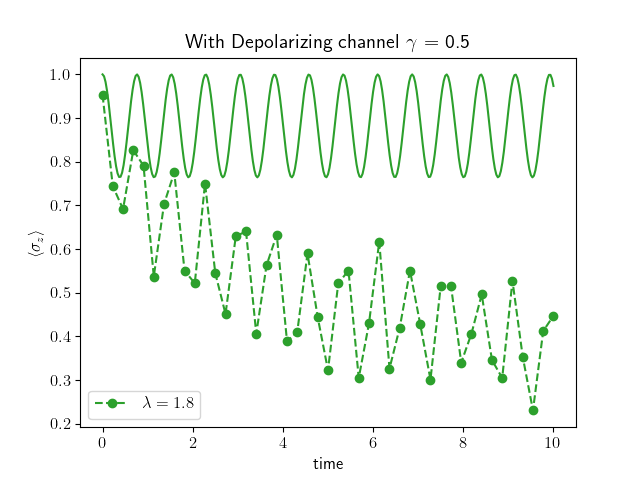
\includegraphics[width=\textwidth]{images/DepolChannelLambda18.png}
    \caption{Time evolution of the Ising model coupled to a depolarizing channel with $\lambda$ = 1.8.%
      \label{fig:DepolChannelLambda18}}
  \end{figure}

  \section{Results}

  \printbibliography
\end{document}


